\documentclass[11pt]{article}
\usepackage{graphicx}
\usepackage{amssymb}
\usepackage{epstopdf}
\DeclareGraphicsRule{.tif}{png}{.png}{`convert #1 `basename #1 .tif`.png}

\textwidth = 6.5 in
\textheight = 9 in
\oddsidemargin = 0.0 in
\evensidemargin = 0.0 in
\topmargin = 0.0 in
\headheight = 0.0 in
\headsep = 0.0 in
\parskip = 0.2in
\parindent = 0.0in

\begin{document}

\subsection*{Synthetic Data Generation for Proximity: Initial Specification\\
Jennifer Neville and Brian Gallagher\\[6pt]
\small{Based on KDL Technical Memo 2004-004\\
2004.09.21 (revised 2004.10.02, 2005.11.30)}
}

\vspace{-1.mm}
\subsection*{Introduction}
\vspace{-4.mm}
A number of KDL research papers have used synthetic datasets to explore hypotheses about the effects of particular data characteristics on estimator, model, and algorithm performance. For example, we have measured the impact of degree on the performance of multiset estimators~\cite{neville-icdm03}, the impact of cluster sizes on classifier performance~\cite{jensen-kdd03}, the impact of attribute correlations on collective inference procedures~\cite{jensen-kdd04}, and the impact of autocorrelation on RDN learning techniques~\cite{neville-icdm04}. Each of these projects has used special purpose python code to generate the data. Now that we have a number of prototypes in python, we would like to add a basic data generation module to Proximity.

In contrast to standard data generation, which typically involves random generation of attribute-value vectors, there are two aspects to generating synthetic relational data. Both the the graph structure (e.g., objects and links) and the attribute values need to be generated. Ideally, we would like a joint model that could generate the relational structure and the attribute values simultaneously but the complexity of such a model makes this approach infeasible. In the first implementation, we will generate the graph structure independently and then generate the attribute values conditioned on the structure. Below we outline generation procedures for two types of graph structures---independent and identically distributed (IID) subgraphs, and homogeneous lattice graphs. Then we outline an attribute generation procedure that can be applied to both types of data. We focus on these two types of graphs because the procedures are relatively easy to implement---in future versions we will want to extend the data generator by adding new methods for generating graph structure and attribute values.

\vspace{-2.mm}
\subsection*{IID Subgraphs}
\vspace{-4.mm}
The first type of graph structure consists of a set of independent bipartite graphs with two object types. For example, consider figure \ref{iid}.

\begin{figure}[ht] 
	\begin{center}
	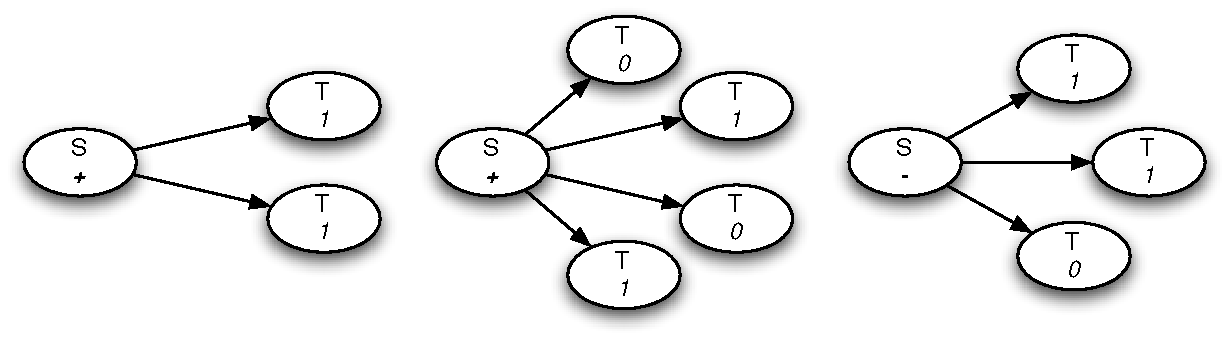
\includegraphics[width=3.75in]{./graphics/synthetic-data}
	\end{center} \vspace{-6.mm}
	\caption{ \label{iid} IID subgraphs.} 
\end{figure} 

\vspace{-3.mm}
\subsubsection*{\emph{Graph Generation}}
\vspace{-5.mm}
The graph generation procedure creates a set of independent subgraphs. There are two object types: S and T. Each subgraph contain a single object S that is connected to a variable number of objects T ($>=0$). Note that each object T links to exactly one object S. The degrees of objects S (i.e., number of linked T objects) in each data set are distributed normally with mean $\mu$ and standard deviation $\sigma$.

\small{
\textbf{Assumptions}
\vspace{-5.mm}
\begin{itemize}
\item There are two object types. We will name the types $S$ and $T$ by convention so users can refer to the object types in their attribute generation parameters.
\item There is a single type of directed link from S to T objects.
\item There are no link attributes.
\end{itemize}
}

\small{
\textbf{User parameters}
\vspace{-5.mm}
\begin{itemize}
\item $N$: number of objects S
\item $P(d_S \: {}_{\widetilde{}} \: N(\mu,\sigma^2))$: probability distribution over degree distributions for objects S
\begin{itemize}
\item For example, degree disparity would specify a set of degree distributions, $P(d_S) = \{N(\mu=10,\sigma^2=1)=0.50, N(\mu=20,\sigma^2=2)=0.50 \}$.
\item For other cases, a single degree distributions in specified, $P(d_S) = \{N(\mu=10,\sigma^2=1)=1.0 \}$.
\end{itemize}
\end{itemize}
}

\small{
\textbf{Generation procedure}
\vspace{-5.mm}
\begin{itemize}
\item For $i$ in $N$
\begin{itemize}
\item Create new object $S_i$
\item Select degree distribution $N_i(\mu, \sigma^2)$ randomly from $P(d_S)$ 
\item Select $d_i$ randomly from the $N_i(\mu, \sigma^2)$ distribution 
	\begin{itemize}
	\item Note that degree needs to be an integer $\geq 0$ so let  $N_i^T=max(0, round(d_i))$ 
	\end{itemize}
\item Create $N_i^T$ objects $T$ and link them to $S_i$
\end{itemize}
\end{itemize}
}

\vspace{-2.mm}
\subsection*{Lattice Graphs}
\vspace{-4.mm}
The second type of graph structure is a homogeneous data graph with a regular square lattice structure. For example, consider figure \ref{lattice}. 
\begin{figure}[ht] 
	\begin{center}
	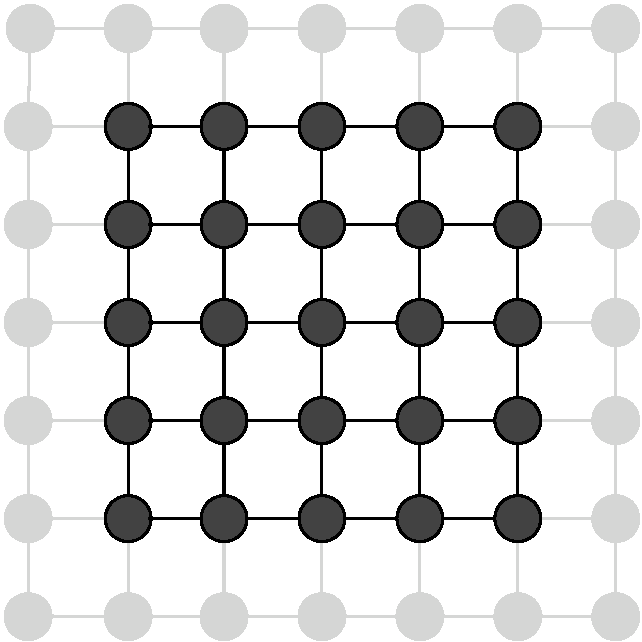
\includegraphics[width=1.5in]{./graphics/lattice}
	\end{center} \vspace{-6.mm}
	\caption{ \label{lattice} Homogeneous lattice graph.} 
\end{figure} 

\vspace{-3.mm}
\subsubsection*{\emph{Graph Generation}}
\vspace{-5.mm}
The graph generation procedure creates a connected graph with a regular lattice structure. There is a single object type S. With the exception of objects along the outer boundary, each object in the lattice links to four immediate neighbors positioned above, below, left, and right. Right now the lattice degree is fixed at $d=4$ but in future versions we may want to make this a user-specified parameter.

\small{
\textbf{Assumptions}
\vspace{-5.mm}
\begin{itemize}
\item There is one object type named $S$ by convention.
\item There is a single type of undirected link among objects S.
\item There are no link attributes.
\end{itemize}
}

\small{
\textbf{User parameters}
\vspace{-5.mm}
\begin{itemize}
\item $N$: number of objects S
\end{itemize}
}

\small{
\textbf{Generation procedure}
\vspace{-5.mm}
\begin{itemize}
\item For $i$ in $\sqrt N$
	\begin{itemize}
	\item For $j$ in $\sqrt N$
		\begin{itemize}
		\item Create new object $S_{ij}$
		\item If $i>0$ link $S_{ij}$ to $S_{(i-1)j}$
		\item If $j>0$ link $S_{ij}$ to $S_{i(j-1)}$
		\end{itemize}
	\end{itemize}
\end{itemize}
}


\vspace{-2.mm}
\subsection*{Attribute Generation}
\vspace{-4.mm}

In IID subgraphs, we generally use the objects S as the target objects to be classified, and objects T are used as peripheral objects during classification. 
Typically, the attribute value generation procedure will assign each object S a single, discrete attribute that will be used as a class label. In order to generate datasets with degree disparity, the assignment of the class labels is conditioned on the degree of the object in the graph. The generation procedure will also add a number of discrete attributes to objects T. The distribution of these attribute values will be conditioned on the class label of the linked object S and the attribute values of neighbors T two links away (to induce autocorrelation). Because the attribute values of one object may depend on the attribute values of related objects, the attribute value generation procedure must assign the attributes ``collectively.''

In lattice graphs, there is a single type of object---objects S are the target objects to be classified, and objects $\leq 2$ links away in the graph are used as peripheral objects during classification. The generation procedure will add a number of discrete attributes to each attribute. Because the attribute values of one object may depend on the attribute values of related objects, again the attribute value generation procedure must assign the attributes ``collectively.''

\small{
\textbf{User parameters}
\vspace{-5.mm}
\begin{itemize}
\item \emph{Prior distributions}
\begin{itemize}
	\item $P_{C_S|d}=P(C_S | d_S)$: conditional probability distribution (CPD) of class given degree
	\item $\mathbf{P_{A_S}}=\{P(A^1_S), ... ,P(A^m_S)\}$: set of prior distributions, one for each of $m$ attributes on objects S
	\item $\mathbf{P_{A_T}}=\{P(A^1_T), ... ,P(A^k_T)\}$: set of prior distributions, one for each of $k$ attributes on objects T
\end{itemize}

\item \emph{Conditional distributions}
\begin{itemize}
	\item $P_{C_S|G}$: CPD for class label, where $G$ is all other data in the graph (e.g., attributes on linked objects S, T, including C)
	\item $\mathbf{P_{A_S|G}}=\{P(A^1_S | G), ... ,P(A^m_S | G)\}$: set of CPDs, one for each of $m$ attributes on objects S
	\item $\mathbf{P_{A_T|G}}=\{P(A^1_T | G), ... ,P(A^k_T | G)\}$: set of CPDs, one for each of $k$ attributes on objects T
\end{itemize}

\item \emph{Other}
\begin{itemize}
	\item $TOL$: tolerance to constrain empirical class distribution 
	\item $iter$: number of Gibbs sampling iterations to use when generating sample
	\end{itemize}
\end{itemize}
}

\vspace{5.mm}
\textbf{Notes}
\vspace{-2.mm}

We can make the class distribution independent of degree for lattice graphs and IID subgraphs by setting $P_{C_S|d}=P(C_S)$.

How can we express the class label CPDs compactly when $d_S$ is drawn from a normal distribution? We could specify probability distributions for ranges of degrees. E.g., $P(C=+|d \in [0,10])=0.50, P(C=+|d \in [11,20])=0.35, P(C=+|d \in [21,\infty])=0.15$.

The tolerance ($TOL$) is used as a loose test on convergence---we use it to throw out samples that are ``far'' from what we expect. For example, generating samples with extreme autocorrelation but uniform class distribution is sometimes difficult to do with Gibbs sampling (from a random initial labeling) because the samples can easily drift to skewed class distributions. In order to limit the variance of our samples we may want to constrain the range of empirical distribution we're willing to accept.

The CPDs can be specified manually in XML---as an RBC or RPT, or any Proximity classifier. Proximity classifiers specify a CPD for a discrete item attribute (e.g., \emph{movie.isBlockbuster}) using a container of subgraphs. The subgraphs identify the relevant related items in the graph. For example, if \emph{linked\_movie.isBlockbuster} is one of the conditioning variables in the CPD, then the model conditions the class probability for each core movie on the class labels of the other items named \emph{linked\_movie} in its subgraph. To simplify the (first) implementation we will assume there are two containers with fixed queries. The first container will be 2d subgraphs (containing all objects $\leq 2$ links away) centered on objects S. By convention we will name the core objects \emph{S}, the objects one link away \emph{linked1\_S} and \emph{linked1\_T}, and the objects two links away \emph{linked2\_S} and \emph{linked2\_T}. The second container will be 2d subgraphs centered on objects T, which follow the same naming convention (although core objects will be named \emph{T}). The manually specified CPDs should follow this convention.

\vspace{5.mm}
\small{
\textbf{Generation procedure}
\vspace{-5.mm}
\begin{itemize}
\item For each object $S_i$
	\begin{itemize}
	\item Randomly assign class label on $S_i$ given 
	the degree of $S_i$ using $P_{C|d_S}$
	\item For $l$ in $m$
		\begin{itemize}
		\item Randomly assign attribute $l$ for object 
		$S_i$, from prior $P(A^l_S)$
		\end{itemize}
	\end{itemize}
\item For each object $T_j$
	\begin{itemize}
	\item For $l$ in $k$
		\begin{itemize}
		\item Randomly assign attribute $l$ for object 
		$T_j$, from prior $P(A^l_T)$
		\end{itemize}
	\end{itemize}
\item Update attribute values using Gibbs sampling: for $h$ in $iter$
	\begin{itemize}
	\item Update the value of the class label for each object $S_i$: 
		\begin{itemize}
			\item Update the value of C for object $S_i$
			by computing a probability estimate with CPD 
			$P_{C_S|G}$ and then randomly assigning a value 
			according to the estimate
		\end{itemize}
	\end{itemize}
	\begin{itemize}
	\item Update the values of each S attribute: for $l$ in $m$
		\begin{itemize}
		\item For each object $S_i$
			\begin{itemize}
			\item Update the value of attribute $l$ for object $S_i$
			by computing a probability estimate with CPD 
			$P_{A^l_S|G}$ and then randomly assigning a value 
			according to the estimate
			\end{itemize}
		\end{itemize}
	\end{itemize}
	\begin{itemize}
	\item Update the values of each T attribute: for $l$ in $k$
		\begin{itemize}
		\item For each object $T_j$
			\begin{itemize}
			\item Update the value of attribute $l$ for object $B_j$
			by computing a probability estimate with CPD 
			$P_{A^l_T|G}$ and then randomly assigning a value 
			according to the estimate
			\end{itemize}
		\end{itemize}
	\end{itemize}
\item Compute the empirical distribution $\hat{P}(C_S)$  
\item If $\hat{P}(C_S) \notin [P(C_S)-TOL,P(C_S)+TOL]$, discard attributes and repeat attribute generation procedure  
\end{itemize}
}

\vspace{-2.mm}
\subsubsection*{Acknowledgments}
\vspace{-4.mm}
Michael Hay and Matt Cornell provided helpful comments on an earlier draft of this memo.

\vspace{-2.mm}
{\small
\renewcommand\refname{\normalsize{References}}
\bibliographystyle{unsrt}
\bibliography{synthetic-data-gen}
}
\end{document} 